\documentclass{article}
\usepackage[margin=1in]{geometry}
\usepackage{tabularx}
\usepackage{hyperref}
\usepackage{enumitem}
\usepackage{graphicx}
\usepackage{parskip}
\usepackage{float}

\title{ \Huge Legislature Bill Organizer \\ \Large User and Administrator manual }
\author{
    Gunnar Knutson \\ \href{mailto://gknutson1@ewu.edu}{gknutson1@ewu.edu} \\ \\
    Steven Harper \\ \href{mailto://sharper12@ewu.edu}{sharper12@ewu.edu} \\ \\
    Ethan Howe \\ \href{mailto://ehowe@ewu.edu}{ehowe@ewu.edu} 
}
\date{Published \today}

\begin{document}
\maketitle
\pagebreak

\begin{table}[h]
    \listoftables
    \addcontentsline{toc}{subsection}{List of Tables}
    \caption{List of Tables}
\end{table}

\begin{table}[h]
    \listoffigures
    \addcontentsline{toc}{subsection}{List of Figures}
    \caption{List of Figures}
\end{table}

\section*{List of Terminology (Glossary)}
\begin{table}[h]
    \def\arraystretch{1.5} % Increase the margins of cells in tables - the default makes them too close together
    \begin{tabularx}{\textwidth}{c X}
        \hline
        Abbreviation & Description \\ 
        \hline
        API & Application/Program Interface. Allows our program to connect to, or be connected to by, other computer programs to facilitate communication. \\
        \hline
        WSL & Washington State Legislature. The governance body that manages the bills we want to track. Provides the data our software utilizes via a public API. \\
        \hline
        SQL & A programming language that is used to interact with databases. \\
        \hline
        MariaDB & A popular database that uses SQL as its primary language to interact with clients. \\
        \hline
        The Database & The MariaDB instance intended for use with any given instance of this program. \\ 
        \hline
    \end{tabularx}
    \def\arraystretch{1}
    \addcontentsline{toc}{subsection}{List of Terminology (Glossary)}
    \caption{List of Terminology}
\end{table}
\pagebreak

\begin{table}[h]
    \tableofcontents
    \addcontentsline{toc}{subsection}{Contents}
    \caption{Table of Contents}
\end{table}
\pagebreak

\section{User's guide}
\label{sec:user}

\subsection{The Main Screen}

\autoref{fig:main} Shows the main screen of the program. This is the landing page when you go to the site, and is where you will navigate to the different parts of the program. At the top of the page is the navigation bar. You can use it to switch between the program's various \textbf{modes}.

\begin{figure}[H]
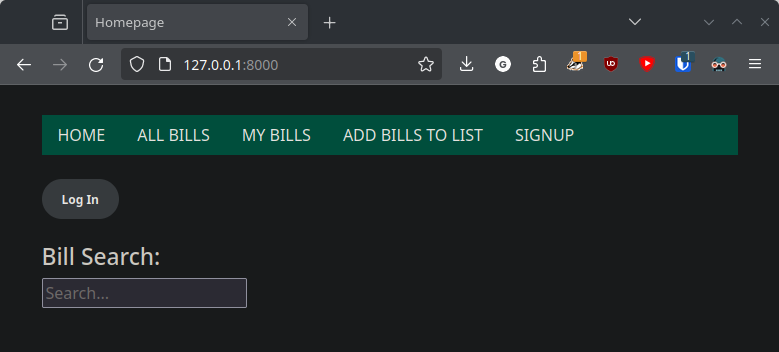
\includegraphics[width=\textwidth]{mainscreen.png}
\caption{Program Main Screen}
\label{fig:main}
\end{figure}

\begin{enumerate}
    \item the \textbf{All Bills} and \textbf{Add Bills} modes display all bills currently in the system, and allow you to take notes on bills and mark bills that you are interested in. There is currently no difference between the two modes, although that my change in the future.
    \item the \textbf{My Bills} mode allows you to view bills that you have marked as having an interest in.
    \item the \textbf{Search} mode (Accessible from the \textbf{Home} tab) allows you to enter search terms to filter bills.
\end{enumerate}

\subsection{Account management}
In order to take notes or access the My Bills view, you must first log in. You can do so by selecting the \textbf{Log In} button on the main page, which will take you to the log in screen (\autoref{fig:login}). Note that, once you have logged in, this button will \textbf{not} disappear.

\begin{figure}[H]
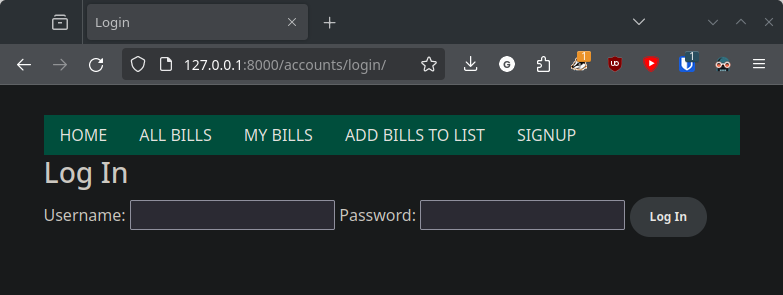
\includegraphics[width=\textwidth]{login.png}
\caption{Login Screen}
\label{fig:login}
\end{figure}

If you do not have an account, you can create one by selecting the \textbf{SIGNUP} option on the navigation bar. This will open the sign up window (\autoref{fig:signup}) which will allow you to create an account with a Username and Password. There is no account recovery system in place, so make sure to safely store this information, or you risk being permanently locked out of your account.

\begin{figure}[H]
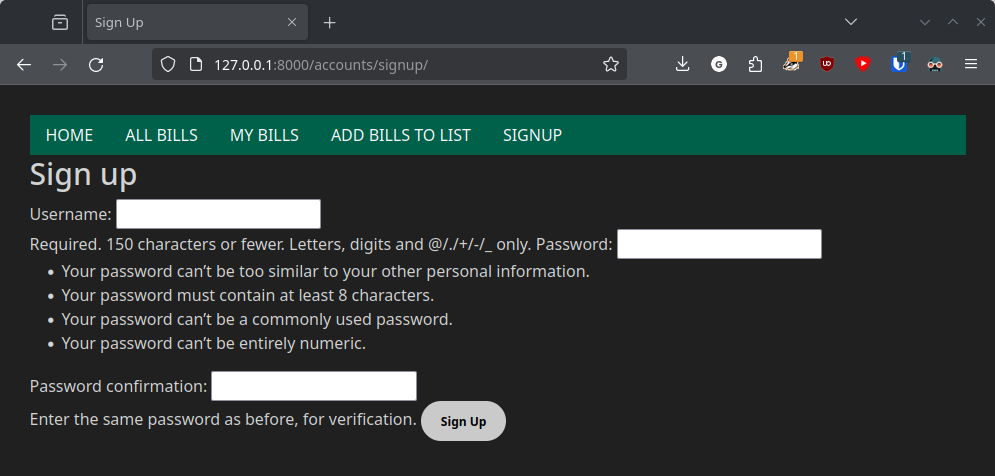
\includegraphics[width=\textwidth]{signup.png}
\caption{Sign Up Screen}
\label{fig:signup}
\end{figure}

\subsection{Viewing bills}

Once you have inserted a search query or selected a bill view from the menu bar, you will be taken to the \textbf{Bills Window} as seen in \autoref{fig:billview}

\begin{figure}[H]
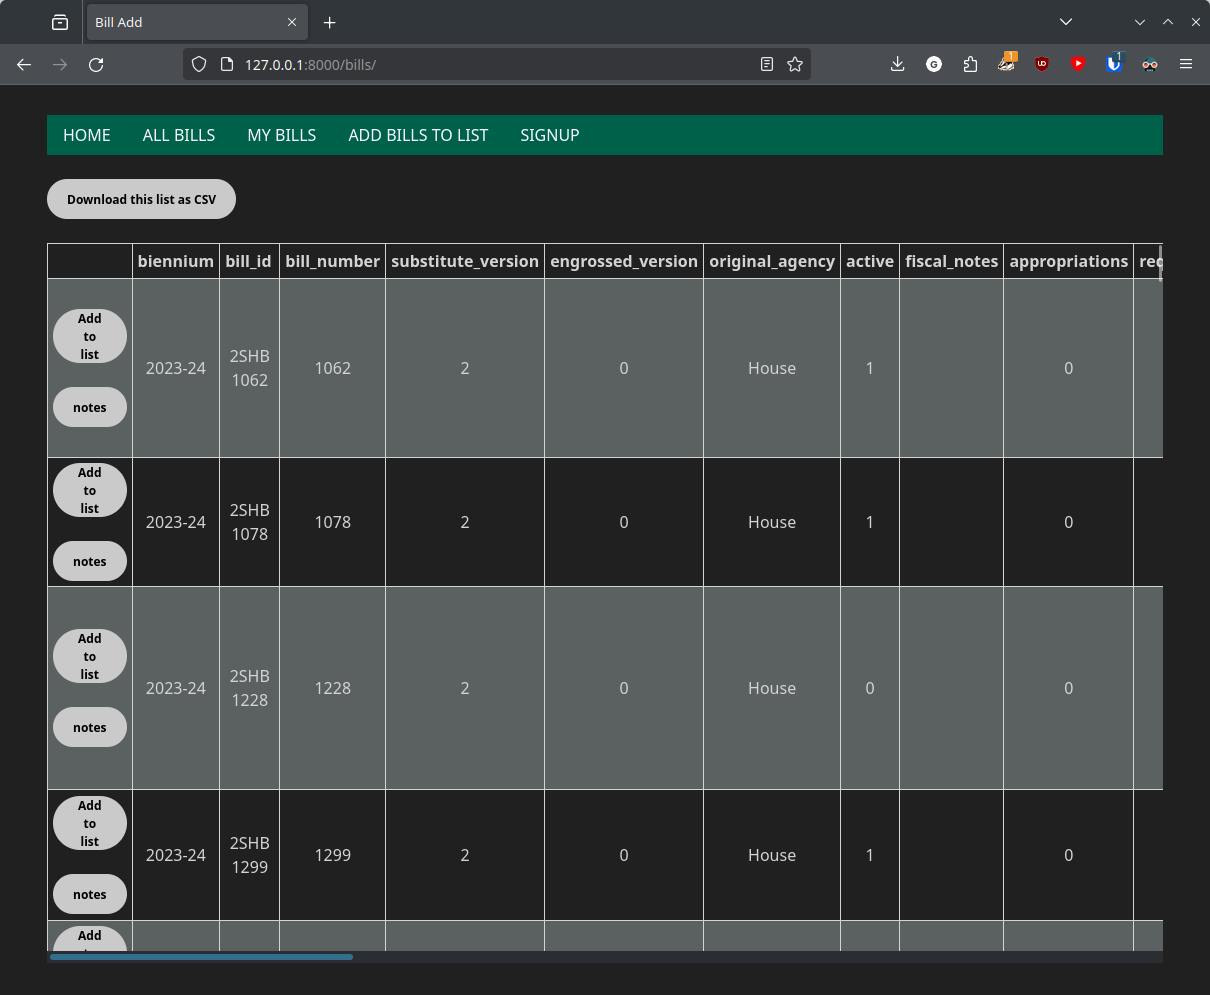
\includegraphics[width=\textwidth]{billview.png}
\caption{Bill View Screen}
\label{fig:billview}
\end{figure}

Note that the \textbf{Add To List} and \textbf{Notes} buttons may not be visible depending on what mode you are in. 

Most computers cannot display the entire bill list at once. In this case, scroll bars on the bottom and left side of the bills window will appear. These bars can be dragged vertically to reveal more bills, or horizontally to reveal more columns.

Selecting \textbf{Add To List} will register the bill so that it will appear when you select the \textbf{My Bills} mode.

\subsection{Note Taking}

The program allows you to write notes on bills. These notes will be saved on the server, and can be viewed at any time. Notes are "connected" to bills, and can be accessed by selecting the \textbf{Notes} button on the left of the desired bill.

\begin{figure}[H]
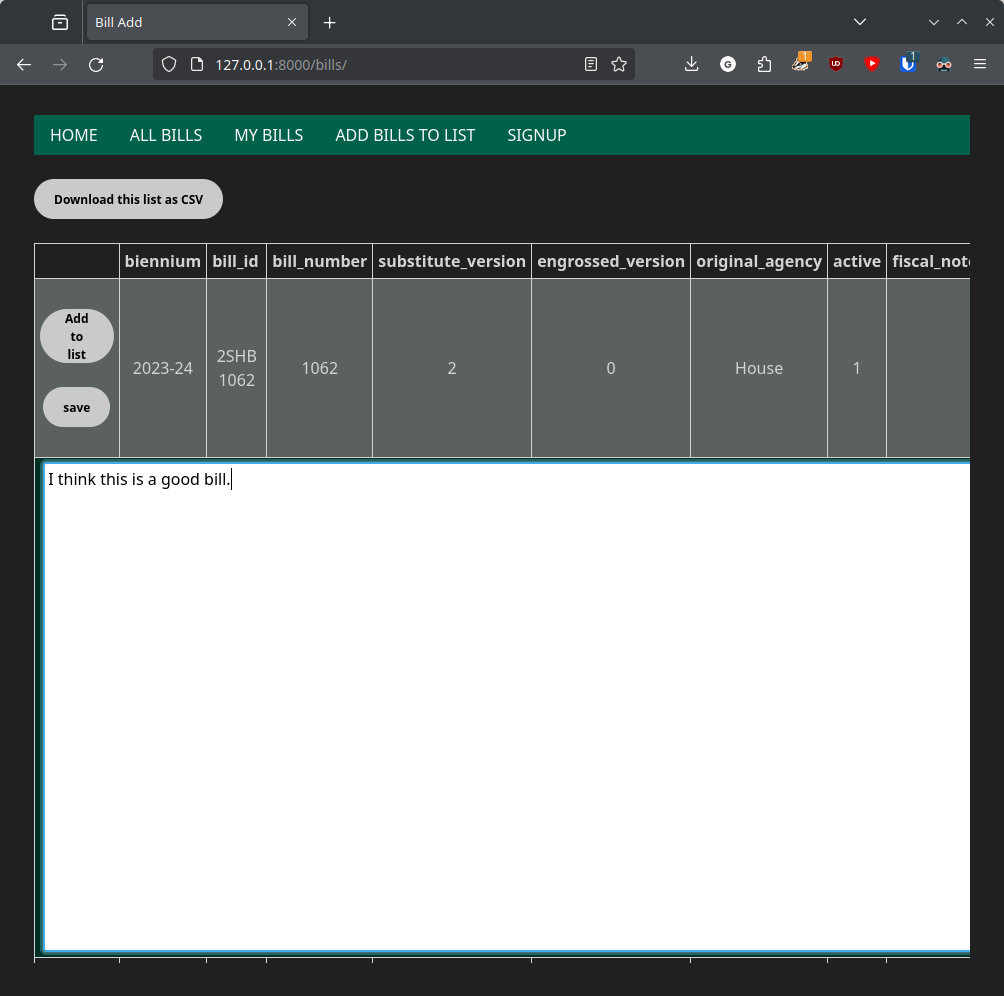
\includegraphics[width=\textwidth]{notes.png}
\caption{Notes Screen}
\label{fig:notes}
\end{figure}

Upon selecting the \textbf{Notes} button, the note will load in a window below the bill, and the button will change into a \textbf{save} button. If you had already written a note for this bill before, the text box will contain what you had previously written. If this is your first time writing a note for this bill, the text box will be blank.

Once you have finished your writing, select the \textbf{save} button. This will save your note to the server and close the note window. If you close the page without selecting \textbf{save} for all notes you have changed, your changes \textbf{WILL BE LOST}.

\subsection{Searching}

You may write search queries into the search bar, seen in \autoref{fig:main}. Once you have entered your query, press \textbf{enter} to preform the search.

Search queries are made up of \textbf{Search Terms}, which are the individual filters that you create, and \textbf{Operations}, which join together search terms and allow adding and removing bills to a search.

\subsubsection{Search Terms}

A search term is made up of three parts: a \textbf{Key}, a \textbf{Operation}, and a \textbf{Value}.

The key determines what data from the bills is retrieved when processing the query.

The operation determines what process is used to determine if a bill passes or fails the query.

The value is what the operation compares against the data in the key.

For instance, If I wanted to find all bills that are active, I would set my key to \textbf{active}, my operation to \textbf{=}, and my value to \textbf{True}, resulting in a search term of \verb"active = True".

Supported operations are \verb"<, >, <=, =>," and \verb"=".

\subsubsection{Operations}

Operations include \verb"&" and \verb"|", and are used for connecting together multiple search terms. When placed between two search terms, \verb"&" allows you to select only bills that match both search terms, and \verb"|" allows you to select bills that match one or both search terms.

\subsection{Downloading}
On every bill view, there is a \textbf{Download this list as CSV} button at the top left section of the screen. Selecting this button will cause your browser to download a file containing all the bills in the current bill view. This list can be imported into software such as a spreadsheet program.

\pagebreak

\section{Administrator's Guide}

This section of the guide is intended for persons who want to run an instance of Legislative Bill Organizer (referred to as "the program" for the remainder of this document) on a personal or production server. If you are a person who wishes to learn how to operate an already operational instance of this software, see the \hyperref[sec:user]{User's guide} section.

\subsection{Requirements}

In order to run the software, you must meet the following minimum requirements:

\begin{enumerate}
    \item An available \href{https://mariadb.org/download/}{MariaDB} instance, of version 10.3 or later. You must have read/write access to this database. This instance will be referred to as "the database" for the remainder of this document.

    \item Access to the Legislative Bill Organizer code. As of the time of writing, the code can be found in the git repository hosted at \href{https://github.com/CSCD488-Winter2024/Bill-Organizer}{github.com/CSCD488-Winter2024/Bill-Organizer}. This code will be referred to as "the repository" for the remainder of this document.

    \item A server to run the program on. This server will be referred to as "the server" for the remainder or this document. The server must meet the following requirements: 
        \begin{enumerate}
            \item \href{https://www.python.org/downloads/}{Python}, of version 3.8 or later.
            \item The ability to install python packages from pip, or all the required python packages installed from alternative sources (see \hyperref[sec:admin:pip]{Python Packages})
            \item \href{https://mariadb.com/downloads/connectors/}{MariaDB C connector}, version 3.3.1 or later.
            \item The ability to communicate with the database via an IP address or hostname.
            \item A copy of the repository. For the rest of the document, it will be assumed that a copy of the repository exists in some folder of the filesystem. This folder will be referred to as \verb_$REPO_. It is assumed that \verb_$REPO_, and all files inside of it, are readable and writable.
            \item It is assumed that the server's operating system is Linux or Linux-related. While the program \textit{theoretically} can be ran on other OSes such as Windows and MacOS, the program has not been tested on other platforms, and is not guaranteed to function properly. The instructions in this document are for Linux systems only, and you will likely have to adapt them if you are not using Linux.
        \end{enumerate}
\end{enumerate}

\subsection{Database Configuration}

This section is about configuring the database itself. For information on connecting the database to the program, see the \hyperref[sec:admin:conf]{Configuration} section.

\subsubsection{Schema}

The program will only use one schema. Is recommended, but not mandatory, to name the schema \verb_billorg_. The schema for the backend bill storage is defined in \verb_$REPO/create-db.sql_. In addition to the tables defined there, several tables will be created for storing user accounts and login information when the program is started up for the first time.

It is recommended that the schema be completeley cleared, and then \verb_$REPO/create-db.sql_ be used to create tables, before the program is started for the first time. While the program \textit{can} create missing tables (see \hyperref[sec:admin:conf]{Configuration}, \verb-create_db-), this feature is inconsistent and may cause issues. 

Note that the program does \textbf{NOT} check at any point if the tables themselves are defined correctly - only whether they exist or not. Correctly defined tables will almost certainty cause undesired behavior, bugs, and crashes.

The schema can be created from the MariaDB console with the following command (where uppercase words should be replaced with their relevant values):

\begin{verbatim}
> mariadb --user=USERNAME --password=PASSWORD --host=HOST --port=PORT SCHEMA < $REPO/create-db.sql
\end{verbatim}

\subsubsection{Permissions}

The software must have read/write access to at least one schema on the database. 
Specifically, the \verb_DELETE_, \verb_SELECT_, and \verb_UPDATE_ privileges must be granted. If the user you wish to use does not have sufficient privileges, you can grant the required privileges from the mariaDB console, where \verb_SCHEMA_ and \verb_USERNAME_ are replaced by the relevant values:

\begin{verbatim}
MariaDB [(none)]> grant delete, select, update on SCHEMA.* to 'USERNAME'@'%'
\end{verbatim}


\subsection{Python Packages}
\label{sec:admin:pip}

All the required Python Packages, as well as their minimum required versions, can be found in the file \verb_$REPO/requirements.txt_. To automatically install all requirements, run the command:
\begin{verbatim}
> pip install -r $REPO/requirements.txt
\end{verbatim} 

Alternatively, your distro may package some or all of these requirements in their package repository. To use these packages, determine the relevant packages by examining \verb_$REPO/requirements.txt_ and your distro's package database, and install them using your distro's package management program. 

Note that both these methods will likely require \verb_sudo_ privlages. If you do not have the relevant permissions or do not wish to use them, consider creating a \href{https://docs.python.org/3/tutorial/venv.html}{python virtual environment}, and use pip to install the requirements in said virtual environment.

\subsection{Configuration}
\label{sec:admin:conf}

The program can load configuration data from environment variables or a \verb"yaml"-formatted config file. Environment variables will override config file variables if both exist. Note that there is some issues with type casting when using environment variables.

The config file must be named \verb"cfg.yml" and be placed in the config directory. The config directory is determined by enironment variables, using the following logic:

\begin{enumerate}
    \item If \verb"BILL_ORGANIZER_HOME", is set, \verb"$BILL_ORGANIZER_HOME"
    \item Else if \verb"XDG_CONFIG_HOME" is set, \verb"$XDG_CONFIG_HOME/bill-organizer"
    \item Else if \verb"LOCALAPPDATA" is set, \verb"$LOCALAPPDATA/bill-organizer"
    \item Else \verb"$HOME/.config/bill-organizer"
\end{enumerate}

See \autoref{table:cfg} for all the possible config values. Note that if no default is shown, the varaible is required.
\begin{table}[h]
    \def\arraystretch{1.5} 
    \begin{tabularx}{\textwidth}{c c c X}
        \hline
        Variable Name & Type & Default & Description \\ 
        \hline
        \multicolumn{4}{c}{\textbf{Database Connection}} \\ 
        \hline
        \verb"db_user" & \verb"str" & & The username of the sql user you are running the program as \\ 
        \hline
        \verb"db_password" & \verb"str" & & The password of the sql user you are running the program as \\ 
        \hline
        \verb"db_database" & \verb"str" & & The schema to use to store bill information \\ 
        \hline
        \verb"db_host" & \verb"str" & & The URL the database can be reached at \\ 
        \hline
        \verb"db_port" & \verb"int" & & The port the database can be reached at \\
        \hline
        \multicolumn{4}{c}{\textbf{Logging}} \\
        \hline 
        \verb"log_level" & \verb"str" & \verb"info" & How detailed to make the logs. Can be \verb"debug", \verb"info", \verb"warning", or \verb"error" \\ 
        \hline 
        \verb"log_format" & \verb"str" & \verb-log-& Format string describing the format of log messages. see Python docs for more info \\ 
        \hline 
        \verb"log_file" & \verb"str" & \verb"None" & When set, logs will be written to the file specified by this variable. Can be a string or a list of path elements. When not set, log info will be printed to stdout. \\ 
        \hline
        \multicolumn{4}{c}{\textbf{General configuration}} \\ 
        \hline
        \verb"name" & \verb"str" & & The name of the program. Should be customized to something unique to you, as this is used to prevent rate limiting by uniquely identifying each instance. \\ 
        \hline 
        \verb"create_db" & \verb"bool" & \verb"False" & If \verb"True", the software will attempt to create any missing tables in the database. If \verb"False", the program will raise an exception if any tables are missing. \\ 
        \hline 
        \verb"init_time" & \verb"int" & \verb"365" & How far back to go to fetch data on bills if a handler has no bills in the database, in days. \\ 
        \hline 
        \verb"wait_time" & \verb"int" & \verb"7" & How long to wait before starting a handler again, in days. Effectively sets the minimum time until an update can take place, as \verb"recheck_delay" and server uptime both have effects on when handlers will actually start. \textbf{MUST} be less than \verb"init_time". \\ 
        \hline 
        \verb"recheck_delay" & \verb"int" & \verb"20" & How many seconds to wait before checking all handlers. Any handlers that need updates will have updates started. \\ 
        \hline 
    \end{tabularx}
    \def\arraystretch{1}
    \caption{Configuration Variables}
    \label{table:cfg}
\end{table}
\end{document}